\chapter{\subspacesTitle}\label{subspacesspanning}

It is time to study vector spaces more carefully and return to  some fundamental questions:

\begin{enumerate}
\item \emph{Subspaces}: When is a subset of a vector space itself a vector space?  (This is the notion of a \emph{subspace}.)

\item \emph{Linear Independence}: Given a collection of vectors, is there a way to tell whether they are independent, or if one is a ``linear combination'' of the others? 

\item \emph{Dimension}: Is there a consistent definition of how ``big'' a vector space is?

\item \emph{Basis}:  How do we label vectors?  Can we write any vector as a sum of some basic set of vectors?  How do we change our point of view from vectors labeled one way to vectors labeled in another way?
\end{enumerate}
\index{Subspace!notion of}\index{Linear independence!concept of}\index{Dimension!notion of}\index{Basis!concept of}
Let's start at the top!

\section{Subspaces}

\begin{definition}
We say that a subset $U$ of a vector space $V$ is a {\bf subspace}\index{Subspace} of $V$ if $U$ is a vector space under the inherited addition and scalar multiplication operations of $V$. 
\end{definition}

\begin{example}
Consider a plane $P$ in $\Re^3$ through the origin:
\[
ax+by+cz=0.
\]

\begin{center}
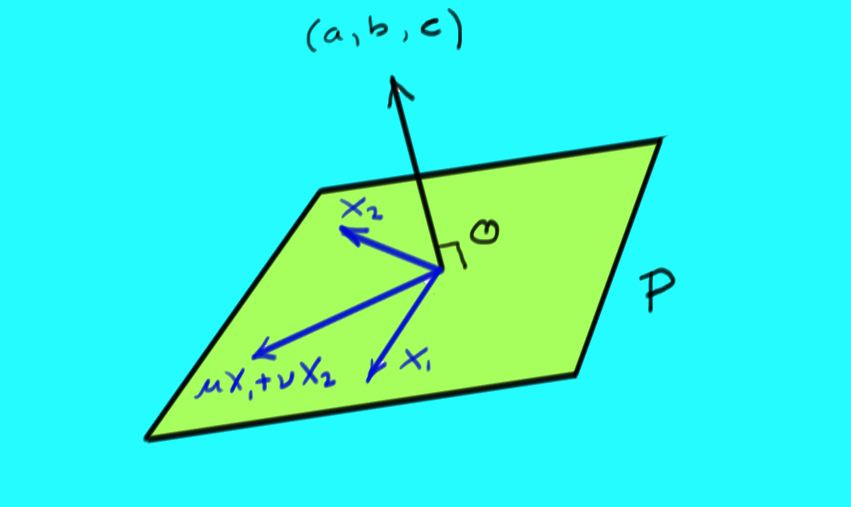
\includegraphics[scale=.3]{\subspacesPath/subspace_plane.jpg}
\end{center}
This equation can be expressed as the homogeneous system $\rowvec{a & b & c}\colvec{x\\y\\z}=0$, or $MX=0$ with $M$ the matrix $\rowvec{a & b & c}$.  If $X_1$ and $X_2$ are both solutions to $MX=0$, then, by linearity of matrix multiplication, so is $\mu X_1 + \nu X_2$:
\[
M(\mu X_1 + \nu X_2) = \mu MX_1 + \nu MX_2 = 0.
\]
So $P$ is closed under addition and scalar multiplication.  Additionally, $P$ contains the origin (which can be derived from the above by setting $\mu=\nu=0$).  All other vector space requirements hold for $P$ because they hold for all vectors in $\Re^3$.
\end{example}


%\begin{figure}
%\begin{center}
%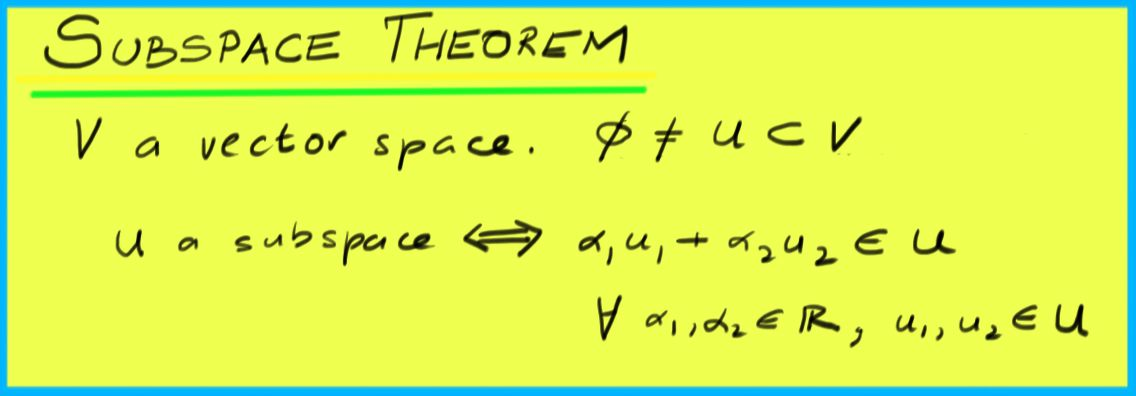
\includegraphics[scale=.33]{\subspacesPath/subspace_thm.jpg}
%\end{center}
%\end{figure}

\begin{theorem}[\hypertarget{sst}{Subspace Theorem}]\index{Subspace theorem}\label{subspacetheorem}
Let $U$ be a non-empty subset of a vector space $V$.  Then $U$ is a subspace if and only if $\mu u_1 + \nu u_2 \in U$ for arbitrary $u_1, u_2$ in $U$, and arbitrary constants $\mu, \nu$.  
\end{theorem}

\begin{proof}
One direction of this proof is easy: if \(U\) is a subspace, then it is a vector space, and so by the additive closure and multiplicative closure properties of vector spaces, it has to be true that \(\mu u_1 + \nu u_2 \in U\) for all \(u_1,u_2\) in \(U\) and all constants constants \(\mu, \nu\).

The other direction is almost as easy: we need to show that if \(\mu u_1 + \nu u_2 \in U\) for all \(u_1, u_2\) in \(U\) and all constants \(\mu, \nu\), then \(U\) is a vector space. That is, we need to show that the \hyperref[vectorspace]{ten properties of vector spaces} are satisfied. We already know that the additive closure and multiplicative closure properties are satisfied. Further, \(U\) has all of the other eight properties  because \(V\) has them. \end{proof}

\noindent
Note that the requirements of the subspace theorem are often referred to as ``closure''\index{Closure}.

%From now on, w
We can use this theorem to check if a set is a vector space. That is, if we have some set \(U\) of vectors that come from some bigger vector space \(V\), to check if \(U\) itself forms a smaller vector space we need check only two things: 
\begin{enumerate}
\item If we add any two vectors in \(U\), do we end up with a vector in \(U\)?
\item If we multiply any vector in \(U\) by any constant, do we end up with a vector in \(U\)? 
\end{enumerate}
If the answer to both of these questions is yes, then \(U\) is a vector space. If not, \(U\) is not a vector space.

%\begin{center}\href{\webworkurl ReadingHomework15/1/}{Reading homework: problem \ref{subspacesspanning}.1}\end{center}
\Reading{SubspacesAndSpans}{1}


\section{Building Subspaces}

Consider the set 
\[
U= \left\{ \colvec{1\\0\\0}, \colvec{0\\1\\0} \right\} \subset \Re^3.
\]
Because $U$ consists of only two vectors, it clear that $U$ is \emph{not} a vector space, since any constant multiple of these vectors should also be in $U$.  For example, the $0$-vector is not in $U$, nor is $U$ closed under vector addition.

But we know that any two vectors define a plane:
\begin{center}
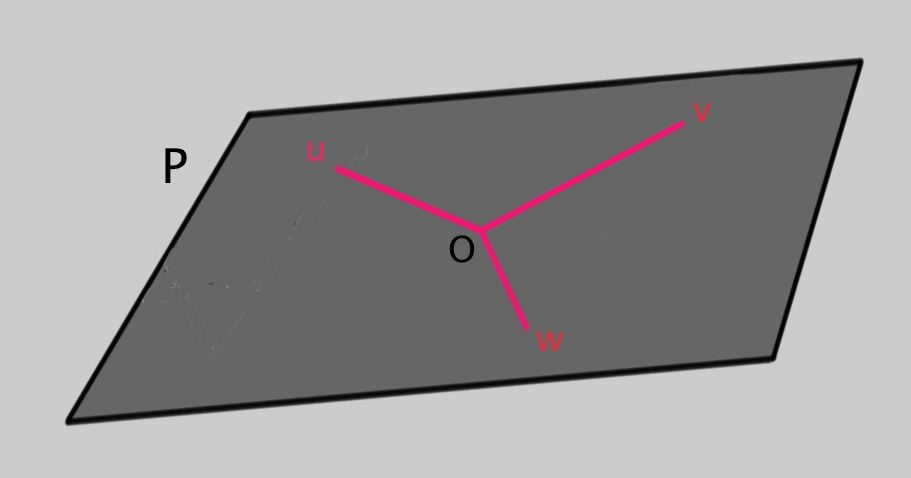
\includegraphics[scale=.3]{\subspacesPath/span_plane.jpg}
\end{center}
 In this case, the vectors in $U$ define the $xy$-plane in $\Re^3$.  We can view the $xy$-plane as the set of all vectors that arise as a linear combination of the two vectors in $U$.  We call this set of all linear combinations the \emph{span}\index{Span} of $U$:
\[
\spa(U)=\left\{ x \colvec{1\\0\\0}+y \colvec{0\\1\\0} \middle| x,y\in \Re \right\}.
\]
Notice that any vector in the $xy$-plane is of the form
\[
\colvec{x\\y\\0} = x \colvec{1\\0\\0}+y \colvec{0\\1\\0} \in \spa(U).
\]

\begin{definition}
Let $V$ be a vector space and $S=\{ s_1, s_2, \ldots \} \subset V$ a subset of~$V$.  Then the {\bf span of $S$}, denoted $\spa(S)$, is the set
\[
\spa(S):=\{ r^1s_1+r^2s_2+\cdots + r^Ns_N ~|~ r^i\in \Re, N\in \N \}.
\]
\end{definition}

That is, the span of \(S\) is the set of all finite linear combinations\footnote{Usually our vector spaces are defined over \(\mathbb{R}\), but in general we can have vector spaces defined over different base fields such as \(\mathbb{C}\) or \(\mathbb{Z}_2\). The coefficients \(r^i\) should come from whatever our base field is (usually \(\mathbb{R}\)).} of elements of \(S\). Any {\it finite} sum of the form ``a constant times \(s_1\) plus a constant times \(s_2\) plus a constant times \(s_3\) and so on'' is in the span of \(S\).\footnote{It is important that we only allow finitely many terms in our linear combinations; in the definition above, \(N\) must be a finite number. It can be any finite number, but it must be finite. We can relax the requirement that $S=\{s_1,s_2,\ldots\}$ and just let $S$ be any set of vectors. Then we shall write $\spa(S):=\{ r^1s_1+r^2s_2+\cdots + r^Ns_N ~|~ r^i\in \Re, s_i\in S, N\in \N, \}$
 }.

\begin{example}
Let $V=\Re^3$ and $X\subset V$ be the $x$-axis.  Let $P=\colvec{0\\1\\0}$, and set $$S=X \cup \{P\}\, .$$
The vector \(\colvec{2 \\ 3 \\ 0}\) is in \(\spa(S),\) because \(\colvec{2\\3\\0}=\colvec{2\\0\\0}+3\colvec{0\\1\\0}.\) Similarly, the vector \(\colvec{-12 \\ 17.5 \\ 0}\) is in \(\spa(S),\) because \(\colvec{-12\\17.5\\0}=\colvec{-12\\0\\0}+17.5\colvec{0\\1\\0}.\)
Similarly, any vector of the form
\[
\colvec{x\\0\\0}+y \colvec{0\\1\\0} = \colvec{x\\y\\0}
\]
is in \(\spa(S)\). On the other hand, any vector in \(\spa(S)\) must have a zero in the \(z\)-coordinate. (Why?) 
So $\spa(S)$ is the $xy$-plane, which is a vector space.  (Try drawing a picture to verify this!)
\end{example}

%\begin{center}\href{\webworkurl ReadingHomework15/2/}{Reading homework: problem \ref{subspacesspanning}.2}\end{center}
\Reading{SubspacesAndSpans}{2}

\begin{lemma}
For any subset $S\subset V$, $\spa(S)$ is a subspace of $V$.
\end{lemma}

\begin{proof}
We need to show that $\spa(S)$ is a vector space.

It suffices to show that $\spa(S)$ is closed under linear combinations.  Let $u,v\in \spa(S)$ and $\lambda, \mu$ be constants.  By the definition of $\spa(S)$, there are constants $c^i$ and $d^i$ (some of which could be zero) such that:
\begin{eqnarray*}
u & = & c^1s_1+c^2s_2+\cdots \\
v & = & d^1s_1+d^2s_2+\cdots \\
\Rightarrow \lambda u + \mu v & = & \lambda (c^1s_1+c^2s_2+\cdots ) + \mu (d^1s_1+d^2s_2+\cdots ) \\
& = & (\lambda c^1+\mu d^1)s_1 + (\lambda c^2+\mu d^2)s_2 + \cdots
\end{eqnarray*}
This last sum is a linear combination of elements of $S$, and is thus in $\spa(S)$.  Then $\spa(S)$ is closed under linear combinations, and is thus a subspace of~$V$.
\end{proof}

Note that this proof, like many proofs, consisted of little more than just writing out the definitions.



\begin{example}
For which values of $a$ does

\[
\spa \left\{ \colvec{1\\0\\a} , \colvec{1\\2\\-3} , \colvec{a\\1\\0}   \right\} = \Re^3?
\]
Given an arbitrary vector $\colvec{x\\y\\z}$ in $\Re^3$, we need to find constants $r^1, r^2, r^3$ such that 

\[
r^1 \colvec{1\\0\\a} + r^2\colvec{1\\2\\-3} +r^3 \colvec{a\\1\\0} = \colvec{x\\y\\z}.
\]
We can write this as a linear system in the unknowns $r^1, r^2, r^3$ as follows:

\[
\begin{pmatrix}
1 & 1 & a \\ 
0 & 2 & 1 \\
a & -3 & 0
\end{pmatrix}
\colvec{r^1\\r^2\\r^3}
= \colvec{x\\y\\z}.
\]
If the matrix $M=\begin{pmatrix}
1 & 1 & a \\ 
0 & 2 & 1 \\
a & -3 & 0
\end{pmatrix}$ is invertible, then we can find a solution 
\[
M^{-1}\colvec{x\\y\\z}=\colvec{r^1\\r^2\\r^3}
\]
for \emph{any} vector $\colvec{x\\y\\z} \in \Re^3$.

Therefore we should choose $a$ so that $M$ is invertible:  

\[
i.e.,\;  0 \neq \det M = -2a^2 + 3 + a = -(2a-3)(a+1). 
\]
Then the span is $\Re^3$ if and only if $a \neq -1, \frac{3}{2}$.
\end{example}

\Videoscriptlink{subspaces_and_spanning_sets_example.mp4}{Linear systems as spanning sets}{scripts_subspaces_and_spanning_sets_example}

Some other very important ways of building subspaces are given in the following examples.

\begin{example}
(The kernel of a linear map).\\[-2mm]

\noindent
Suppose $L:U\to V$ is a linear map between vector spaces. Then if
$$
L(u)=0=L(u')\, ,
$$
linearity tells us that
$$
L(\alpha u + \beta u') = \alpha L(u) + \beta L(u') =\alpha 0 + \beta 0 = 0\, .
$$
Hence, thanks to the subspace theorem,  the set of all vectors in $U$ that are mapped to the zero vector is a subspace of $V$.
It is called the kernel of $L$:
$$
{\rm ker} L:=\{u\in U| L(u) = 0\}\subset U.
$$
Note that finding a kernel means finding a solution to a homogeneous linear equation. 
\end{example}

\begin{example}
(The image of a linear map).\\[-2mm]

\noindent
Suppose $L:U\to V$ is a linear map between vector spaces. Then if
$$
v=L(u) \mbox{ and } v'=L(u')\, ,
$$
linearity tells us that
$$
\alpha v + \beta v' = \alpha L(u) + \beta L(u') =L(\alpha u +\beta u')\, .
$$
Hence, calling once again on the subspace theorem,  the set of all vectors in $V$ that are obtained as outputs of the
map $L$ is a subspace.
It is called the image of $L$:
$$
{\rm im} L:=\{L(u) \ |\  u\in U \}\subset V.
$$
\end{example}

\begin{example}
(An eigenspace of a linear map).\\[-2mm]

\noindent
Suppose $L:V\to V$ is a linear map and $V$ is a vector space. Then if
$$
L(u)=\lambda u \mbox{ and } L(v)=\lambda v\, ,
$$
linearity tells us that
$$
L(\alpha u + \beta v) = \alpha L(u) + \beta L(v) =\alpha L(u) + \beta L(v) =\alpha \lambda u  + \beta \lambda v = \lambda (\alpha u + \beta v)\, .
$$
Hence, again by subspace theorem, the set of all vectors in $V$ that
obey the {\it eigenvector equation} $L(v)=\lambda v$ is a subspace of $V$. 
It is called an eigenspace
$$
V_\lambda:=\{v\in V| L(v) = \lambda v\}.
$$
For most scalars $\lambda$, the only solution to $L(v) = \lambda v$ will be $v=0$, which yields the trivial subspace $\{0\}$.
When there are nontrivial solutions to $L(v)=\lambda v$, the number~$\lambda$ is called an eigenvalue, and carries
essential information about the map~$L$. 
\end{example}

Kernels, images and eigenspaces are discussed in great depth in chapters~\ref{kernelrank} and~\ref{eigenvalseigenvects}.


%\section*{References}
%Hefferon, Chapter Two, Section I.2: Subspaces and Spanning Sets
%\\
%Beezer, Chapter VS, Section S
%\\
%Beezer, Chapter V, Section LC
%\\
%Beezer, Chapter V, Section SS
%\\
%Wikipedia:
%\begin{itemize}
%\item \href{http://en.wikipedia.org/wiki/Linear_subspace}{Linear Subspace}
%\item \href{http://en.wikipedia.org/wiki/Linear_span}{Linear Span}
%\end{itemize}
%

\section{Review Problems}
{\bf Webwork:} 
\begin{tabular}{|c|c|}
\hline
Reading Problems & 
 \hwrref{SubspacesAndSpans}{1}, \hwrref{SubspacesAndSpans}{2}\\
 Subspaces &\hwref{SubspacesAndSpans}{3},
 \hwref{SubspacesAndSpans}{4},
 \hwref{SubspacesAndSpans}{5},
 \hwref{SubspacesAndSpans}{6}\\
 Spans &\hwref{SubspacesAndSpans}{7},
 \hwref{SubspacesAndSpans}{8}\\
  \hline
\end{tabular}






\begin{enumerate}

\item While performing  Gaussian elimination on these augmented matrices write the full system of equations describing the new rows in terms of the old rows above each equivalence symbol as in  \hyperlink{Keeping track of EROs with equations between rows}{Example}~\ref{Rsystem}. 
$$
\begin{amatrix}{2} 
2 & 2 & 10 \\
1 & 2 & 8 \\
\end{amatrix}
,~
\begin{amatrix}{3} 
1 & 1 & 0 & 5 \\
1 & 1 & \!\!-1& 11 \\
-1 & 1 & 1 & -5 \\ 
\end{amatrix}
$$

%%%%%%%%%%%%%%%%%%%

\item Solve the vector equation by applying ERO matrices to each side of the equation to perform elimination. Show each matrix explicitly as in \hyperlink{Undoing}{Example~\ref{slowly}}.

\begin{eqnarray*}
\begin{pmatrix}
3	&6 	&2 \\ %-3
5 	&9 	&4 \\ %1
2	&4	&2 \\ %0
\end{pmatrix} 
\begin{pmatrix}
 x \\ 
y \\
z 
\end{pmatrix} 
=
\begin{pmatrix}
-3 \\ 
1  \\
0  \\
\end{pmatrix} 
\end{eqnarray*}

%%%%%%%%%%%%%%%%%%%

\item Solve this vector equation by finding the inverse of the matrix through $(M|I)\sim (I|M^{-1})$ and then applying $M^{-1}$ to both sides of the equation. 
\begin{eqnarray*}
\begin{pmatrix}
2	&1 	&1 \\ %9
1 	&1 	&1 \\ %6
1	&1	&2 \\ %7
\end{pmatrix} 
\begin{pmatrix}
 x \\ 
y \\
z 
\end{pmatrix} 
=
\begin{pmatrix}
9 \\ 
6  \\
7  \\
\end{pmatrix} 
\end{eqnarray*}


%%%%%%%%%%%%%%%%%%%

\item Follow the method of  \hyperlink{elldeeeww}{Examples~\ref{factorize} and~\ref{factorizes}} to find the $LU$ and $LDU$ factorization of 
\begin{eqnarray*}
\begin{pmatrix}
3	&3 	&6 \\ %0 %2
3 	&5 	&2 \\ %1 %1
6	&2	&5 \\ %0 %1
\end{pmatrix} .
\end{eqnarray*}



%%%%%%%%%%%%%%%%%%%%

\item 
Multiple matrix equations with the same matrix can be solved simultaneously. 
\begin{enumerate}
\item Solve both systems by performing elimination on just one augmented matrix.
\begin{eqnarray*}
\begin{pmatrix}
2	&-1 	&-1 \\ %0 %2
-1 	&1 	&1 \\ %1 %1
1	&-1	&0 \\ %0 %1
\end{pmatrix} 
\begin{pmatrix}
 x \\ 
y \\
z 
\end{pmatrix} 
=
\begin{pmatrix}
0\\ 
1  \\
0  \\
\end{pmatrix} 
,~
\begin{pmatrix}
2	&-1 	&-1 \\ %0 %2
-1 	&1 	&1 \\ %1 %1
1	&-1	&0 \\ %0 %1
\end{pmatrix} 
\begin{pmatrix}
 a \\ 
b \\
c 
\end{pmatrix} 
=
\begin{pmatrix}
2\\ 
1  \\
1  \\
\end{pmatrix} 
\end{eqnarray*}
\item Give an interpretation of the columns of $M^{-1}$ in $(M|I)\sim (I|M^{-1})$ in terms of solutions to certain systems of linear equations.
\end{enumerate}

%%%%%%%%%%%%%%%%%%%%%%%%

\item How can you convince your fellow students to never make this mistake?
\begin{eqnarray*}
\begin{amatrix}{3} 
1 & 0 & 2 & 3 \\ 
0 & 1 & 2& 3 \\
2 & 0 & 1 & 4 \\
\end{amatrix} 
& 
\stackrel{R_1'=R_1+R_2}{
\stackrel{R_2'=R_1-R_2}{ 
\stackrel{\ R_3'= R_1+2R_2}{\sim}}}
&
\begin{amatrix}{3} 
1 & 1 & 4 & 6 \\
1 & \!\!-1 & 0& 0 \\
1 & 2 & 6 & 9 
\end{amatrix}
\end{eqnarray*}

\item Is $LU$ factorization of a matrix unique?  Justify your answer.


\item[$\infty$.] If you randomly create a matrix by picking numbers out of the blue, it will probably be difficult to perform elimination or factorization; fractions and large numbers will probably be involved. To invent simple problems it is better to start with a simple answer:
\begin{enumerate}
\item Start with any augmented matrix in RREF. Perform EROs to make most of the components non-zero. Write the result on a separate piece of paper and give it to your friend. Ask that friend to find RREF of the augmented matrix you gave them. Make sure they get the same augmented matrix you started with.  
\item Create  an upper triangular matrix $U$ and a lower triangular matrix~$L$ with only $1$s on the diagonal. Give the result to a friend to factor into $LU$ form. 
\item Do the same with an $LDU$ factorization. 
\end{enumerate}
\end{enumerate}

\phantomnewpage





\newpage
